\documentclass[tikz,border=5]{standalone}
\usetikzlibrary{backgrounds,arrows.meta}
\usepackage{physics}

\ExplSyntaxOn
\msg_redirect_name:nnn { siunitx } { physics-pkg } { none }
\ExplSyntaxOff

\begin{document}
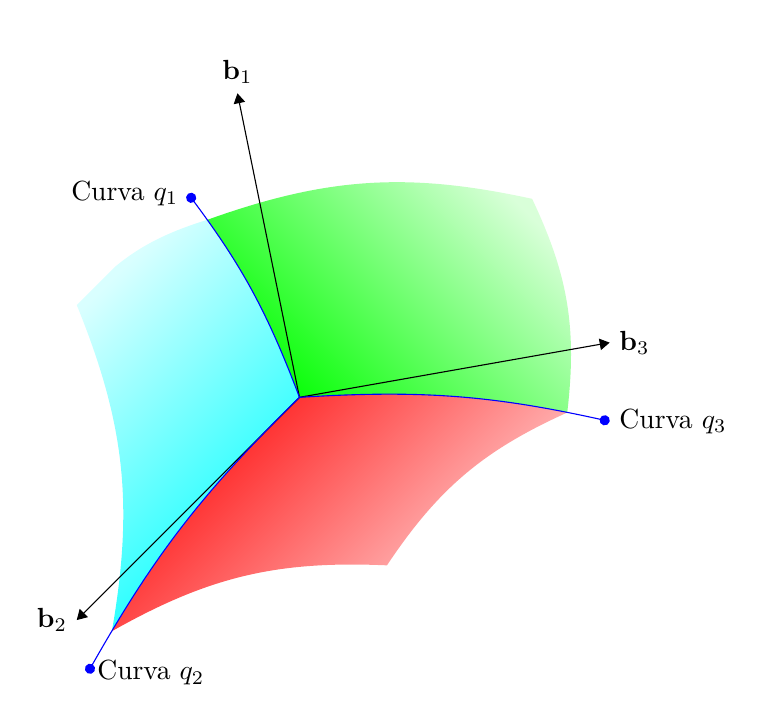
\begin{tikzpicture}[x=(10:4cm),y=(90:4cm),z=(225:4cm),>=Triangle]
  
\coordinate (O) at (0, 0, 0); 

\draw [->] (O) -- (1, 0, 0) node [at end, right] {$\vb{b}_{3}$};

% \draw [->] (O) -- (1, 0.25, 0) node [at end, right] {$\displaystyle \nabla{v}$};

\draw [->] (O) -- (-0.2, 1, 0) node [at end, above] {$\vb{b}_{1}$};
% \draw [->] (O) -- (0.2, 0.7, 0) node [at end, right] {$\displaystyle \nabla{w}$};

\draw [->] (O) -- (0, 0, 1) node [at end, left]  {$\vb{b}_{2}$};
% \draw [->] (O) -- (0.5, 0, 1.1) node [at end, right] {$\displaystyle \nabla{u}$};

\draw [draw=blue, -Circle] (O) to [bend left=8] coordinate [pos=0.875] (q2n) (1, -0.25, 0) coordinate (q2) node [right] {Curva $q_{3}$};

\draw [draw=blue, -Circle] (O) to [bend right=8] coordinate [pos=0.875] (q3n) (0, 1, 0.5) coordinate (q3) node [left] {Curva $q_{1}$};

\draw [draw=blue, -Circle] (O) to [bend right=8] coordinate [pos=0.875] (q1n) (0.25, 0, 1.3) coordinate (q1) node [right] {Curva $q_{2}$};

\begin{pgfonlayer}{background}
\begin{scope}
\clip (O) to [bend left=8] (q2) -- (1, 1, 0) -- (q3n) to [bend right=8] (O);

\shade [left color=green, right color=green!15!white, shading angle=135](O) to [bend left] (q3n) to [bend left=16] (0.75, 0.5, 0) to [bend left=16] (q2n) -- cycle;
\end{scope}

\begin{scope}
\clip (O) to [bend left=8] (q2) -- (1, 0, 1) -- (q1) to [bend left=8] (O);

\shade [left color=red, right color=red!15!white, shading angle=45] (O) to [bend right] (q1n) to [bend left=16] (1, 0, 1) to [bend left=16] (q2n) to [bend right] (O);
\end{scope}

\begin{scope}
\clip (O) to [bend right=8] (q1) -- (0, 1, 1) -- (q3) to [bend left=8] (O);

\shade [left color=cyan, right color=cyan!15!white, shading angle=225] (O) -- (q1n) to [bend right=16] (0, 1, 1) to [bend left=16] (q3n) to [bend left] (O);
\end{scope}
\end{pgfonlayer}


% \node at (0.75, 0.6, 0) {$u(x, y, z) = c_{1}$};
% \node at (0.75, 0.6, 0) {Superficie $q_{2}$};

% \node at (-0.5, 1/2, 1/2) {$v(x, y, z) = c_{2}$};
% \node at (-0.5, 0.5, 0.5) {Superficie $q_{3}$};

% \node at (1.2, 0, 1.2) {$w(x, y, z) = c_{3}$};
% \node at (1.2, 0, 1.2) {Superficie $q_{1}$};
\end{tikzpicture}
\end{document}